% !TeX spellcheck = cs_CZ
\documentclass[a4paper,11pt,titlepage,fleqn]{article}

\usepackage[utf8]{inputenc}
\usepackage[top=3cm, bottom=2.5cm, left=3.5cm, right=2.5cm]{geometry}
\usepackage[czech]{babel}
\usepackage[IL2]{fontenc}  
\usepackage{graphicx}
\usepackage[nonumberlist,acronym]{glossaries}
\usepackage{cite}
\usepackage{fancyhdr}
\usepackage{afterpage}
\usepackage[hidelinks,unicode,hyperfootnotes]{hyperref}
\usepackage{footnote}
\usepackage{parskip}
\usepackage{setspace} 
\usepackage{listings}
\usepackage{pdfpages}
\usepackage{dirtree}
%\usepackage[T1]{fontenc}
%\usepackage[bottom]{footmisc}
%\usepackage{fancyvrb}

\lstset{
    language=PHP,
    basicstyle=\ttfamily\small,
    breaklines=true,
    prebreak=\raisebox{0ex}[0ex][0ex]{\ensuremath{\hookleftarrow}},
    frame=lines,
    showtabs=false,
    showspaces=false,
    showstringspaces=false,
    keywordstyle=\color{red}\bfseries,
    stringstyle=\color{green!50!black},
    commentstyle=\color{gray}\itshape,
    numbers=left,
    captionpos=t,
    escapeinside={\%*}{*)}
}

\renewcommand{\lstlistingname}{Ukázka kódu}
\renewcommand*{\lstlistlistingname}{Seznam zdrojových kódů}

\makeglossaries
\renewcommand*{\glsgroupskip}{}

%\fancyhead[RE,RO]{\textsc{\nouppercase{\leftmark}}}
\rhead{\textsc{\nouppercase{\leftmark}}}
\lhead{}
\pagestyle{fancy}

\addto\captionsczech{\def\refname{Použitá literatura}}
\linespread{1.3}
\setlength{\headheight}{15pt}

\newglossaryentry{tulg}{
    name={Technická univerzita v~Liberci},
    description={Technická univerzita v~Liberci}
}
\newglossaryentry{dp}{
    type=\acronymtype,
    name={DP},
    description={Diplomová práce},
    first={DP}
}

\begin{document}
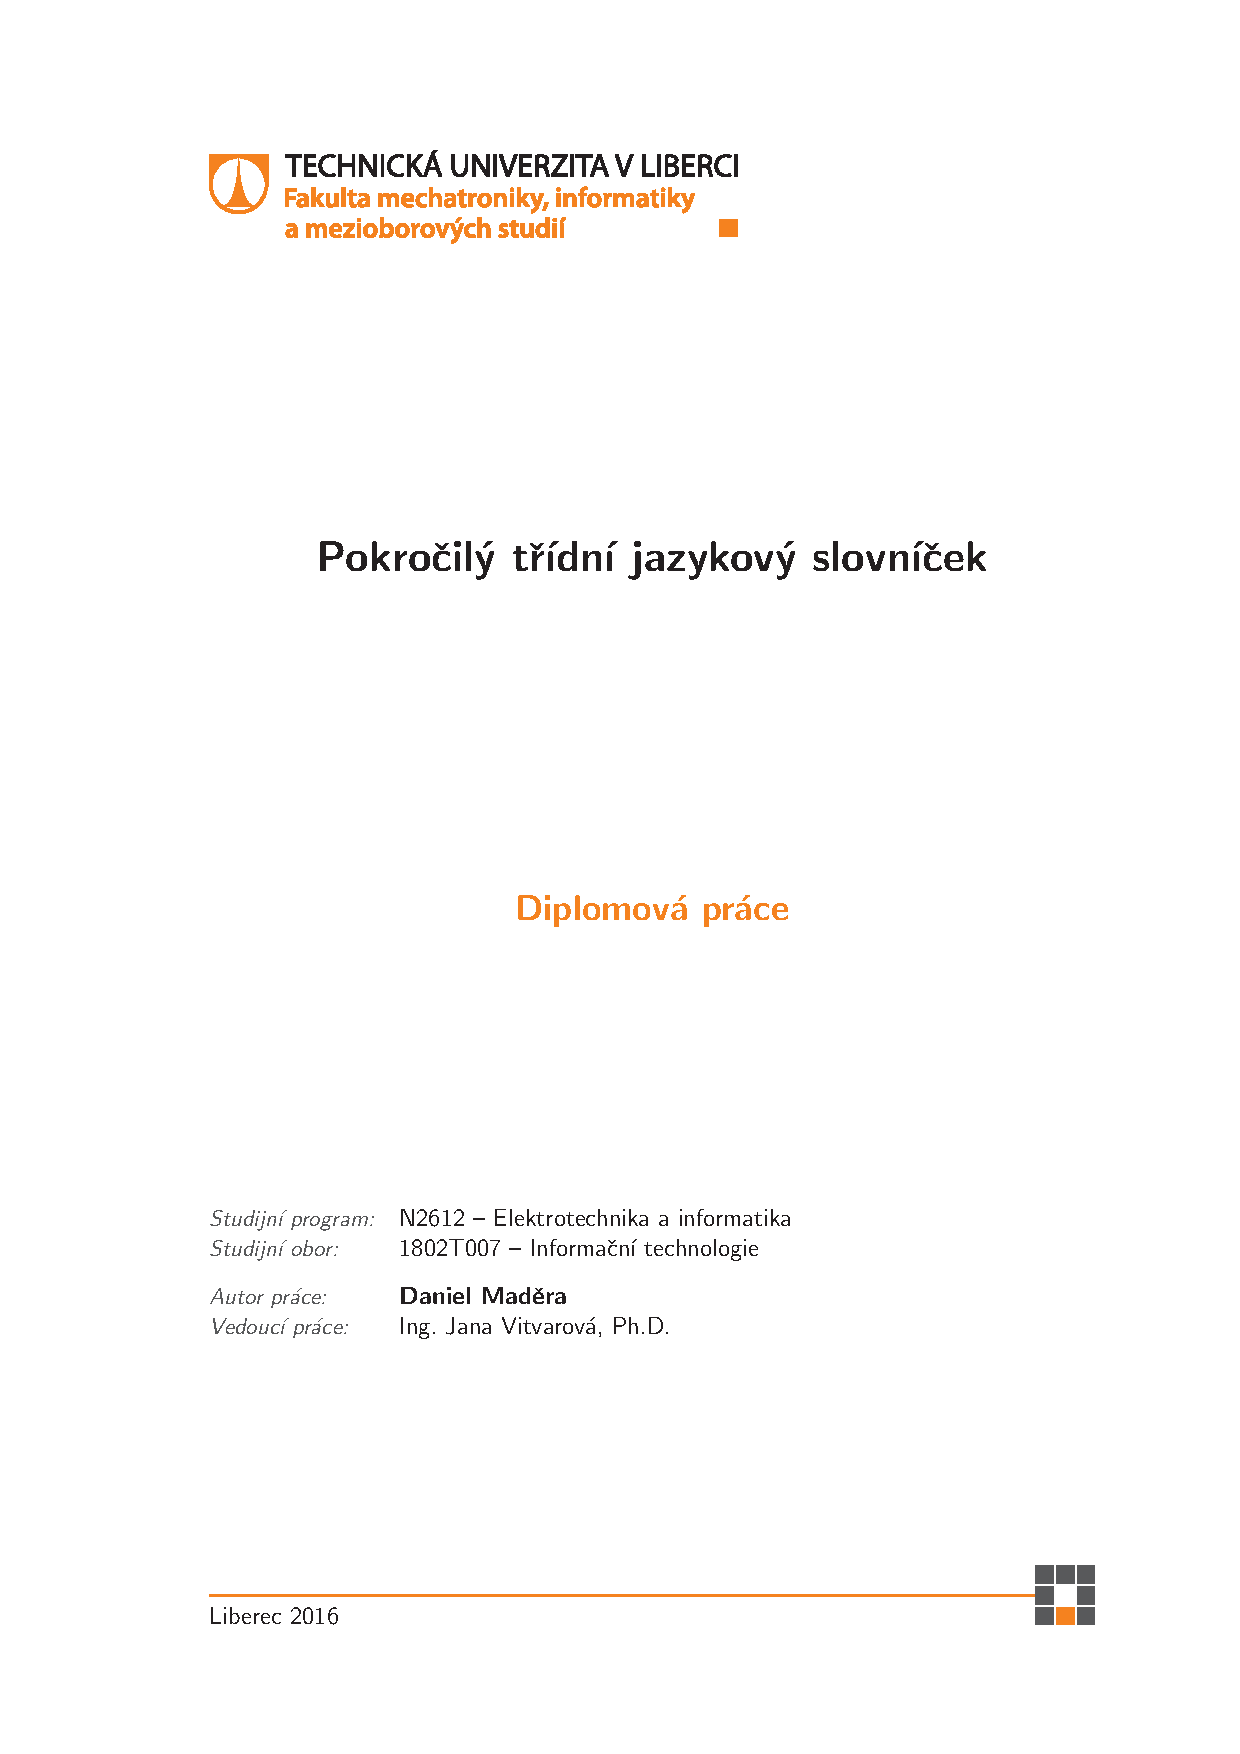
\includepdf[pages={1,2,3}]{dp-titlepage.pdf}
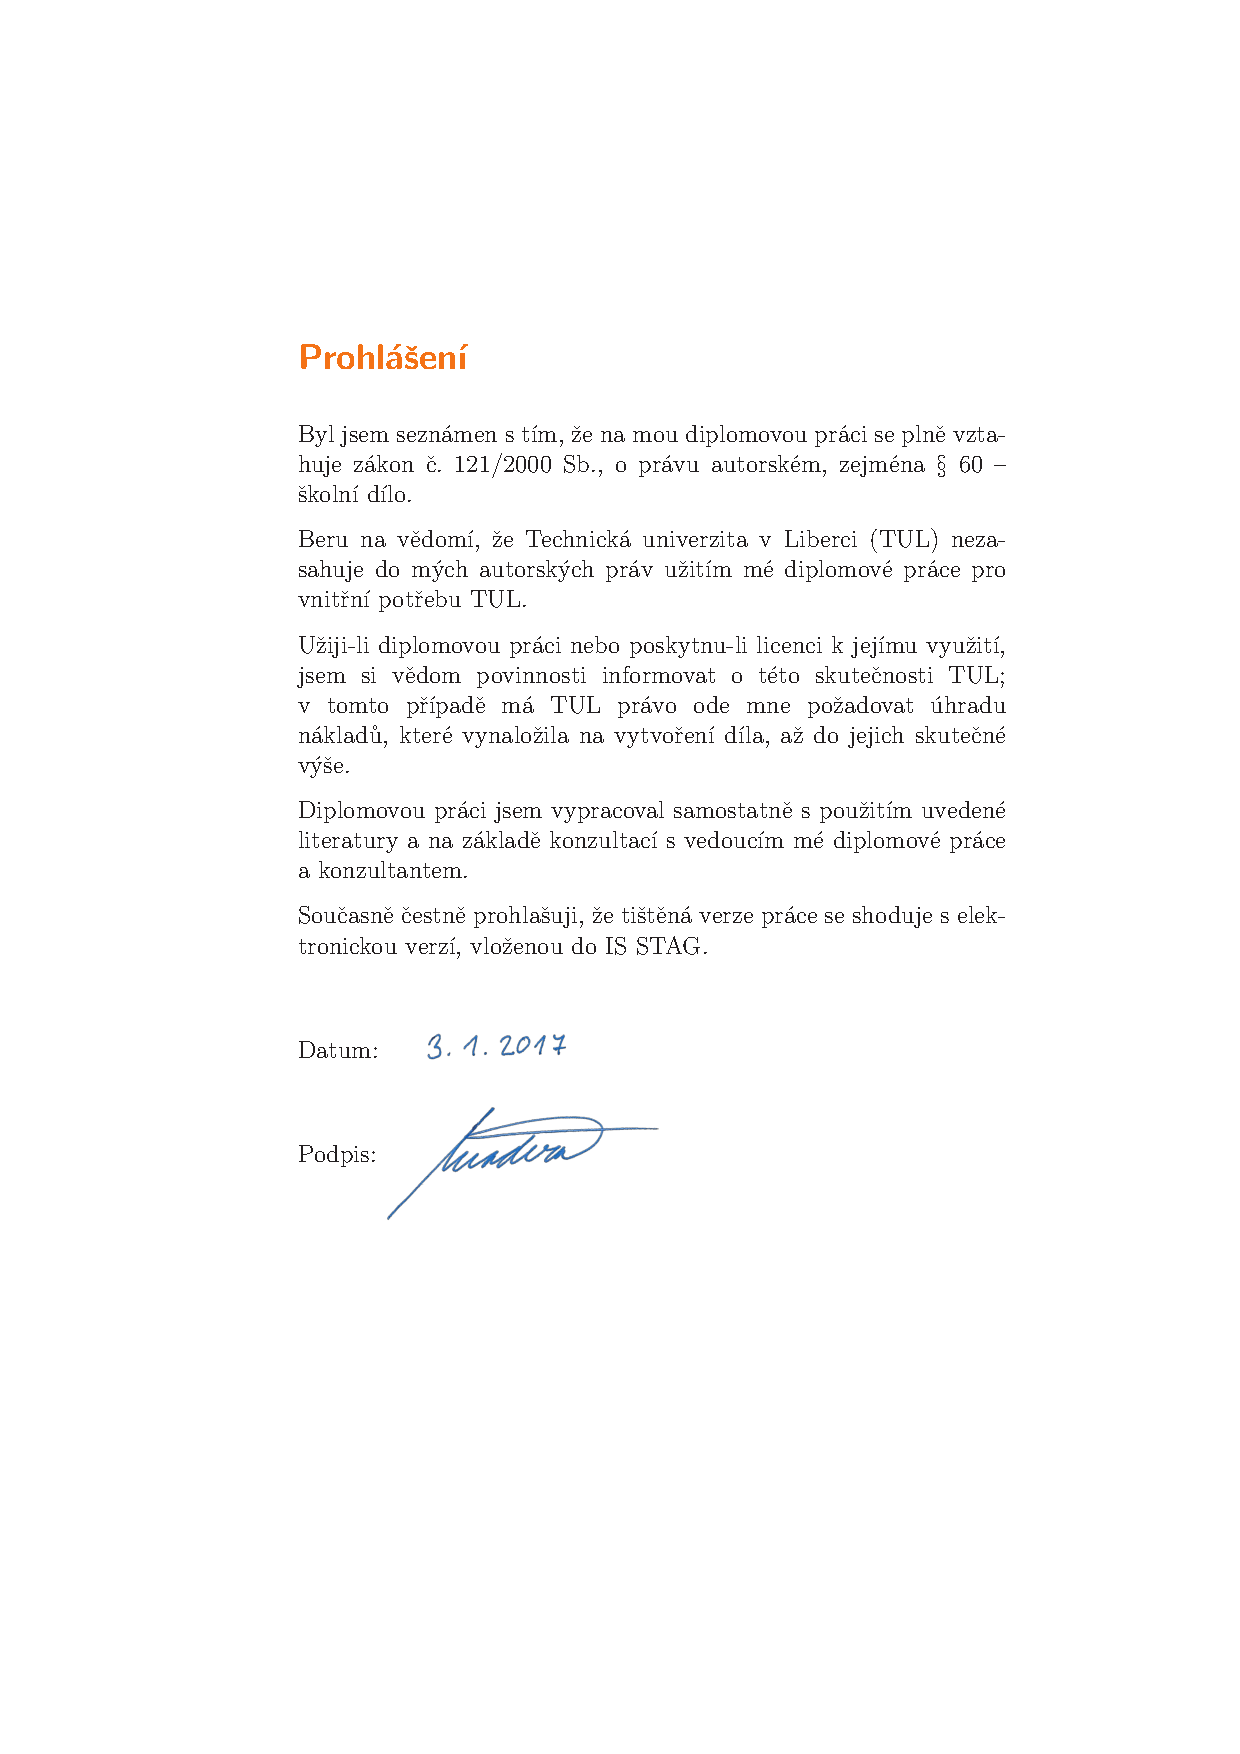
\includepdf{prohlaseni.pdf}
\setcounter{page}{3}

\newpage
\thispagestyle{plain}
\section*{Abstrakt}
% 250 až 500 slov

\section*{Klíčová slova}
% 5 klíčových slov

\thispagestyle{empty}
\newpage

\section*{Abstract}
% 250 až 500 slov

\section*{Keywords}
% 5 klíčových slov

\thispagestyle{empty}

\newpage
\setcounter{tocdepth}{2}
\tableofcontents

\newpage
\listoffigures
\listoftables
\lstlistoflistings

\newpage
\printglossary[type=\acronymtype,title=Seznam zkratek]
%\printglossary[style=altlist,title=Slovník]
\cleardoublepage


\section{Úvod}
    % proč se zaobývat tímto tématem
    % neopakovat abstrakt, lehce nastínit zadání, jaká je motivace
    % popsat, jak je práce strukturovaná - rozcestník


\newpage
\section{Analýza}

    \subsection{Hlavní cíle}
        % jak si aplikaci představuji
        % zlepšení přípravy na hodiny cizího jazyka
        % shrnout v odstavci požadavky na aplikaci
        
        Hlavním cílem aplikace je připravit žáky na hodinu cizího jazyka a zároveň přirozeně rozvíjet slovní zásobu, tak aby studenti neztratili motivaci a chuť k poznávání nových výrazů. Dále také umožnit žákům se protestovat a ověřit, zda naučenou sadu slov ovládají. Aplikace by se měla adaptovat na zdatnost a úroveň každého ze žáků. Vyučujícím by aplikace měla usnadnit správu a import slovíček, které třída má umět v rámci dané učebnice a následně předkládat žákům vhodnou slovní zásobu například pro následující lekci.

        \subsubsection{Personalizace}

            % personalizace podle potřeby konkrétní třídy - konrétní učebnice
            % personalizace podle potřeby jednotlivých žáků - generování na základě předcházejících výsledků

        \subsubsection{Motivace}
            Důležitou součástí vzdělávání obecně je motivace. Tedy přimět žáky, aby z vlastní iniciativy chtěli rozvíjet své vědomosti. Problém ale je, že se děti přirozeně neučí z vlastní iniciativy, ale aby uspokojili okolí. Motivace se rozdělují do skupin - vnitřní a vnější nebo pozitivní a negativní \cite{bib:motivace}. V analýze bude zaměřeno pouze na motivační prostředky, které lze zařadit do aplikace pro procvičování slovíček. 

            Motivace založená na základě vlastních úspěchů je důležitá pro utvrzení sebevědomí žáků. Ocenění v případě zvládnutí sady slov nebo gramatického bloku lze v případě aplikace implementovat například hláškami s projevem pochvaly nebo jiným upozorněním na dosažený výsledek. Zajímavým prvkem v aplikaci by mohlo být i herní prostředí. Žáci si rádi hrají a již J. A. Komenský poukázal na důležitost her ve vzdělávacím procesu.

            % motivace dětí k učení slov (vrámci třídy)
            % motivace - přispění k úspěchu třídy
            % motivace - vlastní úspěchy

            Jedním z dalších stěžejních faktorů motivace je kolektiv. Právě díky kolektivu, ve kterým funguje přirozená rivalita, jsou schopni žáci dosáhnout mnohem vyšších výsledků než kdyby se vzdělávali odděleně a samostatně. Rivalita a soutěživost může projevovat i velmi negativním způsobem. Místo kamarádských vztahů mezi dětmi mohou vznikat nepřátelské, kde může docházet i k posměchu těch, kteří nemusí mít pro výuku až takové nadání. Zajímavější motivací tedy pro kolektiv je například vidina společně dosažených výsledků. V případě učení slovíček by to byl počet slovíček naučených za rok jako celá třída. Dochází zde k utužování kolektivu a děti by mohlo těšit to, že nějakým způsobem přispívají k úspěchům celé třídy.

        \subsubsection{Využití IT pro výuku}
            Posledních několik let se společnost ubírá trendem informačních technologií. Každý ze žáků má už od útlého věku přístup k počítači nebo k chytrému telefonu. Orientace a schopnost tyto zařízení používat není pro ně žádný problém. Přirozeně se tedy tyto zařízení postupně stávají součástí každodenní přípravy žáka na následující školní den. V některých případech tyto zařízení plně nahrazují klasické učebnice a jsou přímo začleněny do výuky. Použití informačních technologií má za následek i zlepšení motivace při výuce. Obecně je známo, že žáci raději studují slovíčka interaktivní formou hádanek, křížovek nebo her, než nekonečných seznamů slov.

            Výuka cizích jazyků je pro aktuální společnost jedna z nejzásadnějších otázek, ať se jedná o pracovní příležitosti v zahraničí, tak sociální problematika světa. Žáci a studenti se často účastní různých kroužků nebo později studenti využívají Erasmus programů, kde vyhledávají právě zlepšení komunikace v cizím jazyce. 
            Důležitost cizích jazyků se projevuje na míře používání například chytrých tabulí nebo tabletů při výuce. Tyto zařízení umožňují interaktivní výuku, kde lze využít nejen textových, ale také obrázkových a zvukových prostředků pro lepší zasazení nově nabytých vědomostí do kontextu. 

            % výuka cizích jazyků - smartboards            
            % vysoká motivace dětí pracovat s PC

    \subsection{Existující řešení}
        Na trhu lze nalézt nepřeberné množství aplikací pro výuku cizích jazyků. Řada z nich jsou téměř komplexní systémy, které provází studenta od základních frází a slovíček až po gramatické standardy cizího jazyka. Analýza existujících řešení byla zaměřena na aplikace, které se zabývají především testováním slovíček a frází.

        Do analýzy existujících řešení byly zahrnuty tři desktopové, jedna webová a jedna mobilní aplikace.

        \subsubsection{TS Angličtina}
            Z analyzovaných řešení se jevila desktopová aplikace TS Angličtina od firmy Terasoft ta nejlépe funkčně propracovaná. Tato firma se zabývám širokou škálou výukových nástrojů se zaměřením na základní školy. V případě cizích jazyků se zabývají výukou anglického a německého jazyka. Hlavní předností aplikace je podpora nejvíce používaných učebnic cizího jazyka. Aplikace umožňuje testování různými způsoby - psaný překlad slova, porozumění mluvenému slovu, vybírání správných významů nebo doplňování vynechaných slov \cite{bib:terasoft}. Analýza byla tvořena pouze z informací vydavatele. Bohužel firma Terasoft neposkytuje DEMO nebo TRIAL verzi aplikace, která by hlubší analýzu umožňovala.

        \subsubsection{Langsoft Teacher}
            Dalším analyzovaným řešením byla aplikace Langsoft Teacher, která je dostupná v podání desktopové aplikace, ale také i mobilní aplikace pro platformy iOS a Android. Aplikace je velmi komplexní, obsahuje různé moduly pro testování například v obrazové formě pro předškolní děti. Zajímavá vlastnost, kterou aplikace disponuje, je pamatování problematických slov a nabízení těchto slov častěji než těch bezproblémových. Dále program umožňuje automaticky rozšiřovat slovní zásobu, která je v testování zahrnuta \cite{bib:langsoft}.

        \subsubsection{Duolingo}
            Dalším v pořadí byla aplikace Duolingo. Jedná se o mobilní aplikaci pro Android. Zahrnuje učivo cizího jazyka od základních komunikačních frází až po tvorbu gramaticky složitějších vět. V aplikaci je připravena dlouhá řada cizích jazyků - němčina, angličtina, španělština (kastilština), italština a další. Chybí ale více referenčních jazyků. Aktuálně lze využít pouze angličtinu. Aplikace kromě standardních funkcí zahrnuje i rozpoznávání mluvených odpovědí. Zajímavým poznatkem byl systém motivace uživatelů, kde si každý mohl pozvat své přátele, mezi kterými docházelo k sdílení dosažených výsledků. Dalším motivačním základem bylo nutkání udržení plánu pravidelného testování, jelikož v opačném případě docházelo k automatickému zvyšování objemu testovacích dat. Nevýhodou aplikace byla nutnost připojení k internetu. V případě požití mobilních dat, docházelo ke zpoždění zejména při rozpoznání slov.

        \subsubsection{Vocabulary Trainer}
            Vocabulary Trainer je webová aplikace zdarma napsaná v jazyce PHP, která naučí 5000 nejvíce používaných slov daného jazyka. Aplikace umožňuje hodně možného nastavení. K dispozici je i řada jazyků včetně češtiny a to jako referenční i jako učený jazyk. Testování spočívá nejdříve ve čtení slov a následně uživatel vybírá možnosti odpovědi. Aktuálně překládané slovo si lze kdykoliv přehrát v různé rychlosti. Jako motivační základ aplikace využívá jednoduchý bodový systém. Součástí je i kalendář s email upomínkou k dalšímu testování. Program je propracovaný, ale poměrně pomalý a dlouho trvá zejména úvodní načítání dat. Její výrobce LanguageCourse S.L. poskytuje i mobilní aplikaci pro Android k učení anglických slov a frází.

        \subsubsection{Supermemo aplikace}
            Za zmínku ještě stojí aplikace Supermemo. Není to aplikace s připravenými daty k testování slov cizího jazyka, ale slouží čistě jako šablona pro testování jakéhokoliv druhu otázek. Aplikace implementuje algoritmus Supermemo, který je založen na metodě postupného zvyšování intervalu dotazování na dané otázky. Při každé odpovědi program spočítá, kdy by si uživatel měl danou otázku zopakovat tak, aby odpověď byla správná a zároveň se co nejvíce zvyšoval interval mezi aktuální a předchozí odpovědí. Aplikace se adaptuje na schopnosti uživatele, v přiměřeném měřítku buď zvyšuje nebo snižuje interval dalšího připomenutí.

        % možné ještě rozvést aplikaci EasyWords

        % žádná z aplikací neumožňuje personalizované učení 
        % ve škole (z učebnice) se učí jiná slovíčka než v aplikacích
        % po otestování slova nedochází k jeho znovu připomenutí

        Z výše uvedených aplikací až na Supermemo žádná neumožňuje personalizovaný výběr učiva. Tedy nelze vložit vlastní slovíčko nebo si určit sadu slov pro testování. Proto jsou tyto aplikace především cílené pro uživatele, kteří vnímají výuku jazyka jako samostatné vzdělávání sami sebe. Pro studenty, kteří absolvují lekce z cizího jazyka ve škole je tento typ vzdělávání nevyhovující, jelikož se musí učit dvě nezávislé skupiny slov. Sice dochází k rozvinutí slovní zásoby studenta i do jiných okruhů než je jeho učebnice a málokterý student má ještě energii, časovou dotaci a vlastní iniciativu na to, aby se připravoval na školní test ze slovíček a ještě rozvíjel samostatně svoji cizojazyčnou slovní zásobu.

    \subsection{Učení slovíček}
        % problematika malých dětí a učení slov
        % Biemiller and Boote (2006)
        % ročně se dá zvládnout maximálně 400 slov u studentů 2 - 5 třídy
        % docházelo k zvýšení učenlivosti, když studenti si mohli zapsat 
        % slovo vlastní definicí

        \subsubsection{Problematika obtížnosti}
        % každý z žáků má indiviální úroveň znalostí cizího jazyka
        % a každý z žádů se jiným tempem učí cizojazyčná slovíčka

        \subsubsection{Učení slov v kontextu}
        % jak je důlžité se slova učit v kontextu - použití ve větě z učebnice
        % drive/vocab-techniques.pdf
    
    \subsection{Testování slovíček}
        % drive/accesing-vocabulary-in-the-language-classroom.pdf
        % důležitost aktivní slovní zásoby pro výuku cizího jazyka

        \subsubsection{Metody testování}
        % pasivní vs aktivní
        % aktivní - vzpomenutí, rozpoznání

        \subsection{Typy testů}
        % multiplechoice, matching, completion, translation
    

    \subsection{Specifikace požadavků}
        % číselný seznam toho, co má aplikace dělat

\newpage
\section{Návrh aplikace}

    \subsection{Uživatelské role a skupiny}
        % usecase diagram
        % jednotlivé use-case by měly být názvy jednotlivých podkapitol v návrhu aplikace
        % rozvést rozdíl mezi žákem a učitelem - rovnocenné partnerství, každý může být učitel a student
    
    \subsection{Učebnice}
        % sdílení učebnic (otevřený systém)
        % přijít do aplikace a jen tak si protestovat slova z učebnice
        % nemusí být člověk součástí žádné skupiny

        \subsection{Hromadný import slovíček}

    \subsection{Interpretace slovíček}
        % výhody více forem - lepší zapamatovatelnost
        % vytvoření hlubších asociací

        \subsubsection{Textová forma}
            % importováním sady slov (bez automatizace překladů)
            % editace definic a použití ve větách

        \subsubsection{Zvuková forma}
            % z Google API importovat zvukové nahrávky
            % shrnout omezení, problematiku

        \subsubsection{Obrazová forma}
            % vyhledání z Google Images API na základě cizojazyčného slova
            % autor učebnice vybírá dané slovo z importovaných
            % omezení dotazů - neprovádí se plně automatiky

    \subsection{Generování slov}
        % shrnout leitnerův algoritmus

        \subsubsection{Rozložené opakování} % Spaced repetition
            % obecně o metodě 

        \subsubsection{Leitnerův algoritmus}

        \subsubsection{Adaptivní a globální obtížnost}

    \subsection{Testování}

        \subsubsection{Metody testování}
            % aktivní rozpoznání a aktivní vzpomenutí
            % algoritmus na záměnu vzpomenutí a rozpoznání (možná obrázek)
    
        \subsubsection{Nápovědy}
            % definice se zobrazuje ihned, kontext slova ve větě z učebnice, první písmeno
            % možnost vyplnění definice slova - (automaticky předvyplnit - volně dostupné definice)

        \subsubsection{Kontrola podvádění}
            % problém, není možné kontrolovat, zda si uživatelé nevyhledávají
            % slova ve slovnících a potom nedoplňují do aplikace
            % měření času odpovědi - v závisloti na délce odpovědi

            % učitel nevidí statistiky dětí, pouze celé třídy
            % aplikace nemá sloužit na zkoušení dětí učitelem
            % testing to learn, not testing to assess        

    \subsection{Vyhodnocování odpovědí}
        % určení vzdálenosti slov - více úrovní odpovědí
        % shrnout levenstein algoritmus

    \subsection{Připomínání slov}
        % shrnout supermemo aplogritmus

    \subsection{Motivace}
        % počty zvládnutých slov studenta
        % třídních zvládnutých slov
        % cinknutí při zvládnutém slově

    \subsection{Architektura aplikace}
        % architektura celé aplikace
        % 2 části, ve skratce popsat, která je za co zodpovědná


\newpage
\section{Klientská aplikace}

    \subsection{Návrh aplikace}

        \subsubsection{Single-page}
            % definice
            % výhody

        \subsubsection{Model aplikace}
            % url diagram
            % mock api

        \subsubsection{Editovatelné seznamy}
            % editace dat v podobě autosave editovatelných seznamů

        \subsubsection{Design}
            % wireframes
            % responzivnost      

        \subsubsection{Implementace algoritmů}
            % Levenstein a Leitner jsou implementovány na klientské straně

    \subsection{Vývojové prostředí}
        \subsubsection{Webpack}
            % css injections, production vlastní css soubor
            % - rychlejší načítání (solo js solo css)

        \subsubsection{Babel}
        \subsubsection{JSX}


    \subsection{Knihovna React}
        
        \subsubsection{Abstraktní DOM}
        \subsubsection{Mobx}
            % knihovna React se stává frameworkem
        \subsubsection{Imutabilita}
        \subsubsection{Směrování}
        \subsubsection{Komponenty}


    \subsection{Implementace technologií}
        % layout komponenta
        % využití Mobx - MVC (stores, components)

        \subsubsection{Adresářová struktura}
        

    \subsection{Testování}
        % Karma, NPM spouštění
        % využití MOBX data injections v daném stavu aplikace


\newpage
\section{Serverová aplikace}
    
    \subsection{Technologie}
        \subsubsection{Webová aplikace}
            % výhody webových aplikací

        \subsubsection{Architektura}
            % architektura klient + server
            % možnost více klientů (mobilní aplikace apod.)

        \subsubsection{HTTP a REST API}

        \subsubsection{WSGI}

        \subsubsection{Implementace algoritmů}
            % Supermemo implementace na serveru
            % CRON připomínací emaily pouze v případě, že stihneš dodělat do APP

    \subsection{Django a REST framework}
        
        \subsubsection{Autorizace}

        \subsubsection{Autentizace}

        \subsubsection{Optimalizace API}

    \subsection{Zabezpečení}

        \subsubsection{HTTP/2}

        \subsubsection{OAuth2}

        \subsubsection{JWT}

        \subsubsection{CORS}

    \subsection{PostgreSQL}

        \subsubsection{DB model}

    \subsection{Testování}
        % APITestCase Django REST


\newpage
\section{Závěr}

\newpage
\begin{thebibliography}{99}
    
    \addcontentsline{toc}{section}{\refname}

    \bibitem{bib:terasoft}
        Terasoft, a.s. \textit{Terasoft - Výukové programy} [online] 2002-10-07. [cit. 2016-12-15]. Dostupné z: \url{http://www.terasoft.cz/czpages/cd_aj15.htm}
    
    \bibitem{bib:langsoft}
        LangSoft s.r.o. \textit{Language Teacher} [online]. [cit. 2016-12-07]. Dostupné z: \url{http://www.langsoft.cz/teacher.htm}

    \bibitem{bib:motivace}
        KREJČOVÁ, L. \textit{Psychologické aspekty vzdělávání dospívajících}. 1. vyd. Praha: Grada Publishing, 2011 [cit 2016-12-18]. ISBN 978-80-247-3474-3.

\end{thebibliography}
\end{document}
